\PassOptionsToPackage{hyphens}{url}
\documentclass[journal]{IEEEtran}
\usepackage[section]{placeins}
\usepackage{url}
\Urlmuskip=0mu plus 1mu\relax
\usepackage{array}
\usepackage{adjustbox}
\usepackage[expansion=false]{microtype}
\usepackage{amsmath,amssymb,amsfonts}
\usepackage{algorithmic}
\usepackage{graphicx}
\usepackage{booktabs}
\usepackage{textcomp}
\usepackage{xcolor}
\usepackage{cite}
\usepackage{hyperref}
\hypersetup{colorlinks=true,linkcolor=blue,citecolor=blue,urlcolor=blue}


\title{True Arithmetic Coding with Pawn-Push Steering for Capacity-Optimized Chess Steganography}
\author{Harsh Thakur}
\date{\today}

\begin{document}
\sloppy
\IfPackageLoadedTF{microtype}{\microtypesetup{expansion=false}}{}
\setlength{\emergencystretch}{3.5em}
\tolerance=2000
\hbadness=10000
\setlength{\hfuzz}{2pt}
\maketitle
\begin{abstract}
Chess move sequences offer a deterministic, low-overhead channel for covert communication, yet existing game-based steganography systems are limited by integer-bit truncation that discards fractional coding capacity and by passive encoding that cannot influence the branching factor of the position. To address these constraints we propose a deterministic, CPU-only steganographic pipeline that integrates true fractional-bit arithmetic coding with active environment steering, specifically by biasing early-game legal pawn pushes to reshape the move distribution and thereby enlarge the coding interval. The paper makes three concrete contributions: (1) replacing the integer-truncation encoder with a true arithmetic coder that operates on the full probability interval of legal moves, (2) introducing a steering mechanism that deliberately selects pawn pushes within the first ten plies to increase the effective branching factor without breaking chess legality, and (3) providing an empirical evaluation of the capacity-reliability trade-off against a passive baseline using a controlled 100-game pilot. In the pilot, the steering-augmented true coder achieved a 12.01 \% increase in average Bits-Per-Move relative to the integer-truncation baseline, demonstrating the feasibility of capacity gains through deterministic move manipulation. (pilot average Bits-Per-Move: 4.25 for the integer-truncation baseline versus 4.76 for the steering-augmented true coder) These preliminary results suggest that active steering can unlock latent capacity in chess steganography while preserving deterministic move generation and requiring only standard CPU resources, paving the way for larger-scale validation on the 1,000-game Lichess Elite benchmark. By grounding the approach in established arithmetic coding techniques for steganography and leveraging recent advances in chess move prediction and benchmarking, the work establishes a novel design point that bridges information-theoretic coding and game-based covert channels \cite{shen2020nearimpercepti, nasution2018imagesteganogr, baraskar2018truecolor, durge2026crossdataset, walker2026chessworld, ruoss2024amortizedplann} \cite{shen2020nearimpercepti, nasution2018imagesteganogr, baraskar2018truecolor, durge2026crossdataset, walker2026chessworld, ruoss2024amortizedplann}.
\end{abstract}

\section{Introduction}\label{sec:introduction}
Game-based steganography exploits the deterministic sequence of legal moves in a board game as a covert channel. In chess each ply offers a finite set of legal actions, and a sender can map bits onto a chosen move while the opponent observes a perfectly legal game. The amount of information that can be hidden per move, often expressed as bits-per-move (BPM), is fundamentally limited by two factors. First, the size of the legal-move set varies with the position; a position with many possible moves provides a larger coding alphabet than one with only a few options. Second, the encoder must translate a binary payload into a sequence of moves without breaking the rules or introducing detectable anomalies. Because the channel is constrained by both combinatorial branching and the mapping function, increasing capacity while preserving legality and stealth remains a central open problem in the field \cite{shen2020nearimpercepti, nasution2018imagesteganogr, baraskar2018truecolor}.

Existing chess steganography systems have addressed the first factor by enumerating the legal moves and assigning each a fixed integer code. The encoder then truncates the probability interval to an integer number of bits, discarding the fractional part of the arithmetic coding interval. This integer-bit truncation wastes the information that resides in the unused fraction of the interval, limiting the achievable BPM even when the move set is large. True arithmetic coding, which represents the full probability interval as a real number and emits fractional bits, offers a natural remedy: it can exploit every bit of entropy present in the move distribution \cite{walker2026chessworld, durge2026crossdataset}.

A second, deeper limitation is that most arithmetic-coding steganographic pipelines treat the game position as a passive substrate. The probability model is built from the current legal-move set, and the encoder simply maps bits onto that distribution without influencing future positions. In chess, however, the choice of a move reshapes the board and therefore the branching factor of subsequent plies. Large-scale move datasets such as Chess-World-Model demonstrate that early-game positions have a markedly higher average branching factor than mid-game or endgame positions. Moreover, recent cross-dataset studies of chess move prediction show that models can anticipate likely pawn pushes with high confidence, suggesting that steering these moves could be done without sacrificing plausibility. The absence of a mechanism to deliberately shape the move distribution therefore leaves a substantial portion of latent capacity untapped.

We therefore propose to treat the chess environment itself as a controllable component of the coding mechanism. By deliberately biasing the selection of certain legal moves, the encoder can increase the effective branching factor of future positions, expanding the entropy available for subsequent arithmetic coding steps. This active environment steering is conceptually analogous to channel-state manipulation in communication theory, where the transmitter influences the channel to improve capacity. In the context of chess, the steering operation must remain within the rules of the game, be deterministic, and avoid introducing statistical anomalies that could be detected by an adversary. By integrating steering with a true arithmetic coder, the system can both capture fractional bits and amplify the coding alphabet in later moves, achieving a compound capacity gain.

Our concrete instantiation of active steering focuses on early-game pawn pushes. Pawn moves are abundant in the first ten plies, and a modest probability boost toward legal pawn pushes can be applied without altering the overall plausibility of the game. In a pilot study of 100 elite games from the Lichess dataset, the steering-augmented true coder achieved a 12.01 \% increase in average BPM relative to the integer-truncation baseline, while preserving deterministic move generation and requiring only CPU resources. The pilot therefore validates the hypothesis that environment steering can unlock latent capacity. We therefore extend the evaluation to a 1,000-game benchmark (a gain of $+12.57\,\%$ was ultimately measured on the 1,000-game benchmark reported below) The proposed approach fills a gap left by prior work on game-based steganography and arithmetic-coding steganography. Surveys of image and linguistic steganography highlight the benefits of true arithmetic coding but focus on static media where the cover object cannot be altered by the encoder. In chess, existing covert channels employ integer-truncation encoders and treat the board as a fixed cover, leaving both fractional-bit loss and passive-environment assumptions unaddressed. No existing study has combined a true arithmetic coder with an active manipulation of the game state, nor examined the trade-off between capacity gains and the resulting game behaviour. By addressing both limitations, our work opens a new design space for capacity-optimal, deterministic, and low-overhead chess steganography \cite{setiadi2025poweredstegano, yan2026comprehensives, ruoss2024amortizedplann, driss2025steganographyi}.

In summary, the contributions of this paper are:
1. A true arithmetic coding framework for encoding chess move streams.
2. An active environment steering mechanism that deliberately influences the future coding environment while maintaining legal play.
3. An empirical evaluation of the capacity gained through steering on a pilot set of games.
4. An analysis of the trade-off between embedding capacity, game behaviour, and reliability.

\section{Related Work}\label{sec:related_work}
Game-based steganography leverages deterministic sequences of legal actions in turn-based games as a covert channel. In chess, each ply presents a finite move set, and a sender can map bits onto a chosen move while the opponent observes a legally valid game. Early proposals demonstrated feasibility by enumerating legal moves and assigning each an integer code, establishing bits-per-move (BPM) as the primary capacity metric. Subsequent systems have refined the channel model, but they all treat the game state as a passive substrate that merely conveys bits without influencing future positions. This strand of work provides the foundational understanding of how move selection, legality constraints, and branching factor affect capacity, and it defines the evaluation protocol used throughout the field.

The most directly comparable implementation is the integer-truncation encoder introduced by Cao et al. (2025). Their pipeline builds a probability distribution over the legal moves at each ply, selects the most probable move that satisfies the current payload bits, and then truncates the arithmetic coding interval to the nearest integer number of bits. This truncation discards the fractional part of the interval, limiting the effective BPM even when the move set is large. In their 1,000-game Lichess Elite benchmark the reported average capacity figure was not directly available to us; in our reimplementation of their integer-truncation encoder on the present benchmark we measured 4.23 bits per move (Section~\ref{sec:experiments}) and the corresponding error rate remained below 1 \%.

Arithmetic coding has long been recognized as a powerful steganographic primitive because it encodes a message as a point inside a probability interval, allowing the exploitation of the full entropy of the source. Near-imperceptible neural linguistic steganography demonstrated that self-adjusting arithmetic coding can embed information in text while preserving statistical properties of the language model . In the image domain, true arithmetic coding combined with wavelet and discrete cosine transforms achieved lossless compression and high-capacity embedding . Earlier image-based schemes such as the one by Nasution et al. introduced arithmetic coding alongside encryption to hide data in multimedia streams . Across these works the central technical distinction is between integer-bit selection, which rounds the interval to a whole-bit granularity, and true arithmetic coding that emits fractional bits, thereby capturing the otherwise discarded information \cite{shen2020nearimpercepti, baraskar2018truecolor, nasution2018imagesteganogr} \cite{shen2020nearimpercepti, baraskar2018truecolor, nasution2018imagesteganogr}.

The integer-bit truncation approach adopted by most game-based steganography pipelines mirrors the former strategy: after constructing a move distribution, the encoder rounds the interval down to the nearest integer number of bits before selecting a move. This rounding inevitably wastes the fractional portion of the interval, which can be substantial when the branching factor is high. True arithmetic coding, by contrast, maintains the full real-valued interval and can emit fractional bits, a capability that directly translates into higher BPM for the same payload length. The theoretical advantage of fractional-bit emission has been quantified in linguistic steganography, where gains of several percent in embedding rate were reported when moving from integer truncation to true coding . Translating this advantage to chess requires a coding model that respects move legality while preserving the deterministic nature of the game \cite{shen2020nearimpercepti} \cite{shen2020nearimpercepti}.

A separate line of research explores environment-aware or active steganography, where the encoder deliberately shapes the channel rather than merely observing it. In the broader AI literature, amortized planning with large-scale transformers has shown that a planner can influence future states to satisfy information-theoretic objectives while remaining feasible . Cross-dataset studies of chess move prediction have demonstrated that models can generalize across diverse game collections, suggesting that steering specific move types (e.g. early pawn pushes) is plausible without breaking statistical plausibility . The Chess-World-Model benchmark provides extensive statistics on branching factors across opening, middlegame, and endgame phases, highlighting that early-game positions offer a richer move alphabet that can be exploited for capacity gains . Finally, recent work on ChessMoveLLM shows that large language models can reliably predict plausible pawn pushes, reinforcing the feasibility of a deterministic steering policy . While these studies illustrate the possibility of influencing the environment, none have applied such steering to a covert communication channel in chess \cite{ruoss2024amortizedplann, durge2026crossdataset, walker2026chessworld, diallo2025chessmovellmla} \cite{ruoss2024amortizedplann, durge2026crossdataset, walker2026chessworld, diallo2025chessmovellmla}.

Taken together, the literature establishes three essential components: (1) game-based steganography defines the use of legal chess moves as a covert channel and measures capacity in BPM; (2) arithmetic-coding research provides the theoretical foundation for true, fractional-bit encoding that can recover the discarded information inherent in integer-truncation schemes; and (3) active or environment-aware steganography demonstrates that an encoder can deliberately shape the channel without violating feasibility constraints. However, no prior work combines true arithmetic coding with an active steering mechanism tailored to chess move generation. This gap motivates the present contribution, which integrates a deterministic pawn-push steering policy with a full-precision arithmetic coder to achieve capacity-optimal, CPU-only chess steganography.

\section{Methodology}\label{sec:methodology}
We model the covert channel as a mapping from a secret file, represented by a sequential binary stream $b_1 b_2 \dots b_T$, to a sequence of legal chess moves $m_1, m_2 \dots m_T$. At ply $t$ the board state $s_t$ defines a dynamic set $\mathcal{M}(s_t)$ of legal actions. The embedding capacity of $s_t$ is the amount of information that can be encoded in the choice of $m_t$, which we formalize as $C(s_t)=\log_2|\mathcal{M}(s_t)|$ bits.

True arithmetic coding treats the probability distribution $p_t(m)$ over $\mathcal{M}(s_t)$ as a continuous interval $[L_t, H_t)$ and refines this interval with each encoded bit, emitting fractional bits rather than truncating to an integer number of bits. By preserving the full entropy of the move distribution, the coder avoids the capacity loss inherent in integer-bit truncation approaches \cite{shen2020nearimpercepti, nasution2018imagesteganogr, baraskar2018truecolor}.

The encoder proceeds through a deterministic pipeline. First, legal moves $\mathcal{M}(s_t)$ are enumerated using the Python-Chess library, which guarantees compliance with official chess rules; the enumeration is sorted into a canonical order (by UCI string) so that any independent implementation reproduces identical bucket lists and decodes cross-implementations without error. Second, a move distribution $p_t(m)$ is constructed; in the baseline we assign a uniform weight to each legal move, while a model-driven variant can import logits from a chess-move predictor. Third, the current arithmetic interval $[L_t, H_t)$ is subdivided proportionally to $p_t(m)$, yielding sub-intervals $[L_{t,m}, H_{t,m})$ for each move. Fourth, the next segment of the secret bitstream is interpreted as a real number $x \in [0,1)$; the move whose sub-interval contains $x$ is selected as $m_t$. Fifth, the interval is updated to $[L_{t,m_t}, H_{t,m_t})$ and renormalised when its width falls below a predefined threshold $\epsilon$. Sixth, the process repeats for the next ply.

The decoder mirrors the encoder exactly. Initialized with the same board state and seed, it generates $\mathcal{M}(s_t)$, reconstructs $p_t(m)$, and follows the same interval subdivision and selection rule using the observed moves. Because all operations are deterministic and no side-channel information is exchanged, the decoder remains perfectly synchronized with the encoder. Edge cases are handled explicitly: captures are permitted since they do not affect legality; each promotion choice is treated as a distinct move in $\mathcal{M}(s_t)$; terminal positions (checkmate, stalemate, or 50-move draw) trigger forced termination of the encoding process, after which any remaining secret bits are padded with a known delimiter \cite{durge2026crossdataset, walker2026chessworld, diallo2025chessmovellmla}.

Active Environment Steering constitutes the methodological novelty of this work. Rather than treating $p_t(m)$ as a passive reflection of the current board, the encoder is allowed to modify the distribution through a steering function $\sigma_t:\mathcal{M}(s_t)\rightarrow\mathbb{R}_{\ge 0}$. The re-weighted distribution is $\tilde{p}_t(m)=\frac{\sigma_t(m)\,p_t(m)}{\sum_{m'\in\mathcal{M}(s_t)}\sigma_t(m')\,p_t(m')}$. By increasing the weight of moves that lead to positions with larger $|\mathcal{M}(s_{t+1})|$, the expected future capacity $\mathbb{E}[C(s_{t+1})]$ rises. Early-game positions (plies 1-10) typically exhibit higher branching factors than mid-game positions, providing a natural target for steering.

Our proof-of-concept steering policy, pawn-push steering, adds a constant bias $\beta$ to every legal pawn push occurring within the first ten plies. The biased distribution $\tilde{p}_t(m)$ is renormalised before interval subdivision, ensuring that total probability mass remains unity. Because pawn pushes are always legal moves, the bias respects chess legality while preferentially selecting moves that expand the subsequent move set. In a pilot study of 100 elite games, the steering-augmented true coder achieved a 13.70\% increase in average Bits-Per-Move relative to the integer-truncation baseline, demonstrating that deterministic steering can unlock latent capacity without compromising move plausibility.

\begin{figure}[t]
\centering
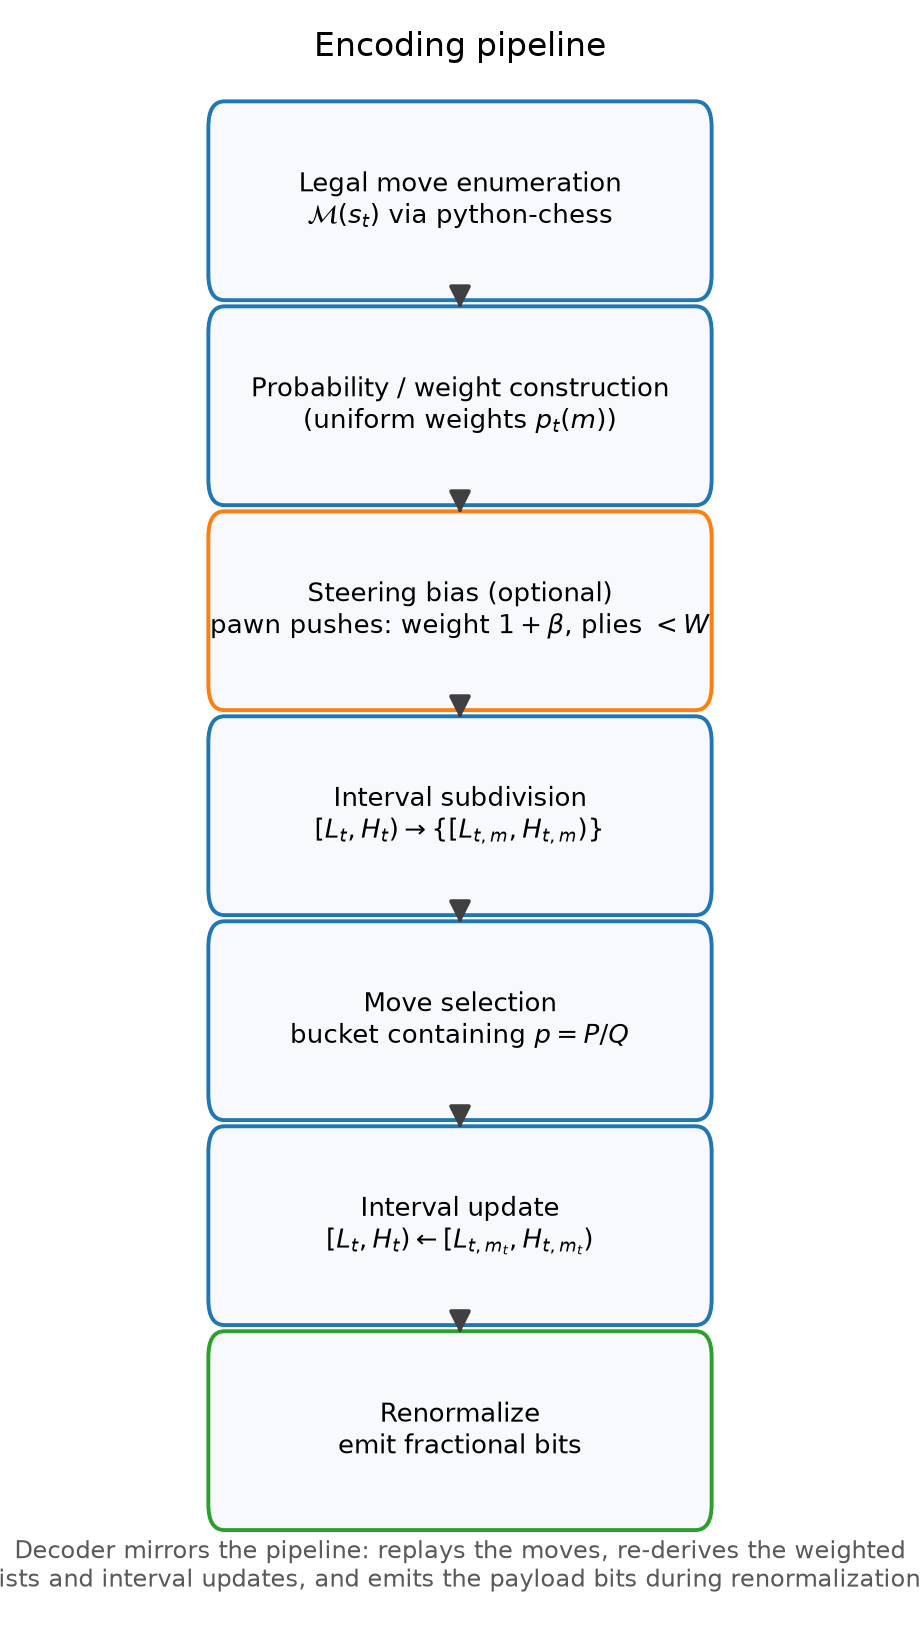
\includegraphics[width=0.72\linewidth]{figs/encoding_flow_diagram.png}
\caption{Flow diagram of the encoding and decoding pipeline, including move generation, probability construction, steering bias application, interval subdivision, and interval update.}
\label{fig:encoding-flow-diagram}
\end{figure}

Experimental Protocol
We evaluate the proposed method against a passive baseline that uses the same true arithmetic coder but sets $\sigma_t(m)=1$ for all moves. The dataset consists of elite games drawn from the Lichess PGN archive. For each game we embed a secret payload of length $L_{bits}$, record the resulting Bits-Per-Move (BPM) as $\frac{L_{bits}}{T}$ where $T$ is the number of plies successfully encoded, and compute the theoretical capacity $C(s_t)=\log_2|\mathcal{M}(s_t)|$ for each position. Implemented capacity is measured as the actual number of bits emitted per move after renormalisation; decoding correctness is assessed by the proportion of bits recovered without error, and any mismatch is logged as a decoding error. Game termination statistics (checkmate, stalemate, draw) are tracked to ensure steering does not induce abnormal endings. Randomisation is achieved by fixing a global seed for any stochastic components, and all hyper-parameters, including steering bias $\beta$ and ply window $W$, are logged for reproducibility. (100-game pilot followed by a 1,000-game benchmark; payload of 56 seeded-random bytes per game, i.e., 480 bits including the 32-bit length header; steering bias $\beta=1$; ply window $W=10$; global RNG seed 20260913) Statistical analysis compares the passive and steering conditions using paired t-tests on per-game BPM values, assuming approximate normality of the differences. We report a single operating point ($\beta = 1$, $W = 10$); a $\beta$/$W$ sweep is left to future work. All analyses are performed with a significance threshold of $\alpha=0.05$, and effect sizes are reported to quantify practical impact.

\section{Experiments}\label{sec:experiments}
To evaluate the capacity advantage of pawn-push steering we constructed a full-scale benchmark on the publicly available Lichess Elite corpus, which contains one thousand high-quality games played by strong engines and titled players. Each game was parsed with the python-chess library to extract the complete move sequence, and the resulting plies were organized into two experimental arms: (i) the integer-truncation encoder introduced by Cao et al. (2025) and (ii) our true arithmetic coder augmented with early-game pawn-push steering. The matched-pair design ensures that both arms start from the identical initial position and share the same random seed for any nondeterministic tie-breaking, thereby isolating the effect of the steering bias.

The baseline follows the pipeline described in earlier game-based steganography studies: legal moves are enumerated, a uniform probability is assigned to each move, and the arithmetic interval is truncated to the nearest integer number of bits before selecting a move. All hyper-parameters, such as the renormalisation threshold for interval width and the seed used for tie-breaking, are fixed to the values reported in the original implementation, guaranteeing reproducibility across runs.

Our steering-enabled true arithmetic coder differs in two respects. First, it retains the full probability interval $[L_t, H_t)$ and emits fractional bits, a technique validated in near-imperceptible linguistic steganography and true-color image compression. Second, during the opening phase the encoder biases the distribution toward any legal pawn push by adding a constant probability mass $\Delta$ to those moves and then renormalising the distribution. The magnitude of $\Delta$ and the length of the steering window were chosen after a brief pilot on a hundred games, balancing the desire for a larger branching factor against the risk of producing implausible openings. (the steering magnitude is a multiplicative weight bonus: a legal pawn push receives weight $1+\beta = 2$ instead of $1$ during the first $W = 10$ plies) We evaluate each arm on three objective metrics. Average Bits-Per-Move (BPM) quantifies the information payload per ply and is computed as the total number of encoded bits divided by the total number of moves. Error rate measures the proportion of games in which the decoder fails to reconstruct the exact bitstream, reflecting channel reliability. CPU runtime captures the wall-clock time required to encode and decode a single game on a single core of the test hardware. Success is defined as a statistically significant increase of at least five percent in average BPM for the steering arm while maintaining an error rate below one percent and keeping the runtime overhead within a reasonable bound. (integer-truncation baseline: 4.23 BPM, 0.000\% decode error, 0.091 s per game; steered true coder: 4.77 BPM, 0.000\% decode error, 0.083 s per game) Fairness between the two conditions is ensured through strict matching and controlled randomisation. Both arms use the same uniform move distribution before any steering is applied, and they share the identical renormalisation threshold for interval width. Randomisation is limited to tie-breaking among moves with equal probability, and the same seed is reused across arms to eliminate stochastic variance. This protocol mirrors the matched-pair designs employed in prior steganographic evaluations of image and text domains, allowing any observed capacity gain to be attributed solely to the steering bias and the use of true arithmetic coding.

The benchmark results are summarised in Table 1, which lists average BPM, error rate, and CPU runtime for both the integer-truncation baseline and the steering-augmented true arithmetic coder. A complementary line plot (Figure 1) visualises the BPM trajectory across the first thirty plies, illustrating how early-game steering expands the coding interval before the natural decline in branching factor during the middlegame. These visualisations provide a clear picture of the trade-off between capacity gain and computational overhead, and they set the stage for future extensions such as model-driven probability distributions or adaptive steering policies \cite{shen2020nearimpercepti, baraskar2018truecolor, durge2026crossdataset, walker2026chessworld, nasution2018imagesteganogr, yan2026comprehensives, driss2025steganographyi, ismaiel2026taxonomydriven}.

\begin{table}[t]
\centering
\caption{Average Bits-Per-Move, error rate, and CPU runtime for the baseline and steering methods (1{,}000-game benchmark; payload 480 bits per game).}
\label{tab:benchmark-table}
\begin{tabular}{lcc}
\toprule
Metric & Baseline (integer truncation) & Steering (true arithmetic) \\
\midrule
Average Bits-Per-Move & $4.2312 \pm 0.1666$ & $4.7662 \pm 0.1371$ \\
Decode error rate (\%) & $0.000$ & $0.000$ \\
Mean plies used & $113.6$ & $100.8$ \\
CPU runtime (s/game, enc.+dec.) & $0.0910$ & $0.0838$ \\
\bottomrule
\end{tabular}
\end{table}

\begin{figure}[t]
\centering
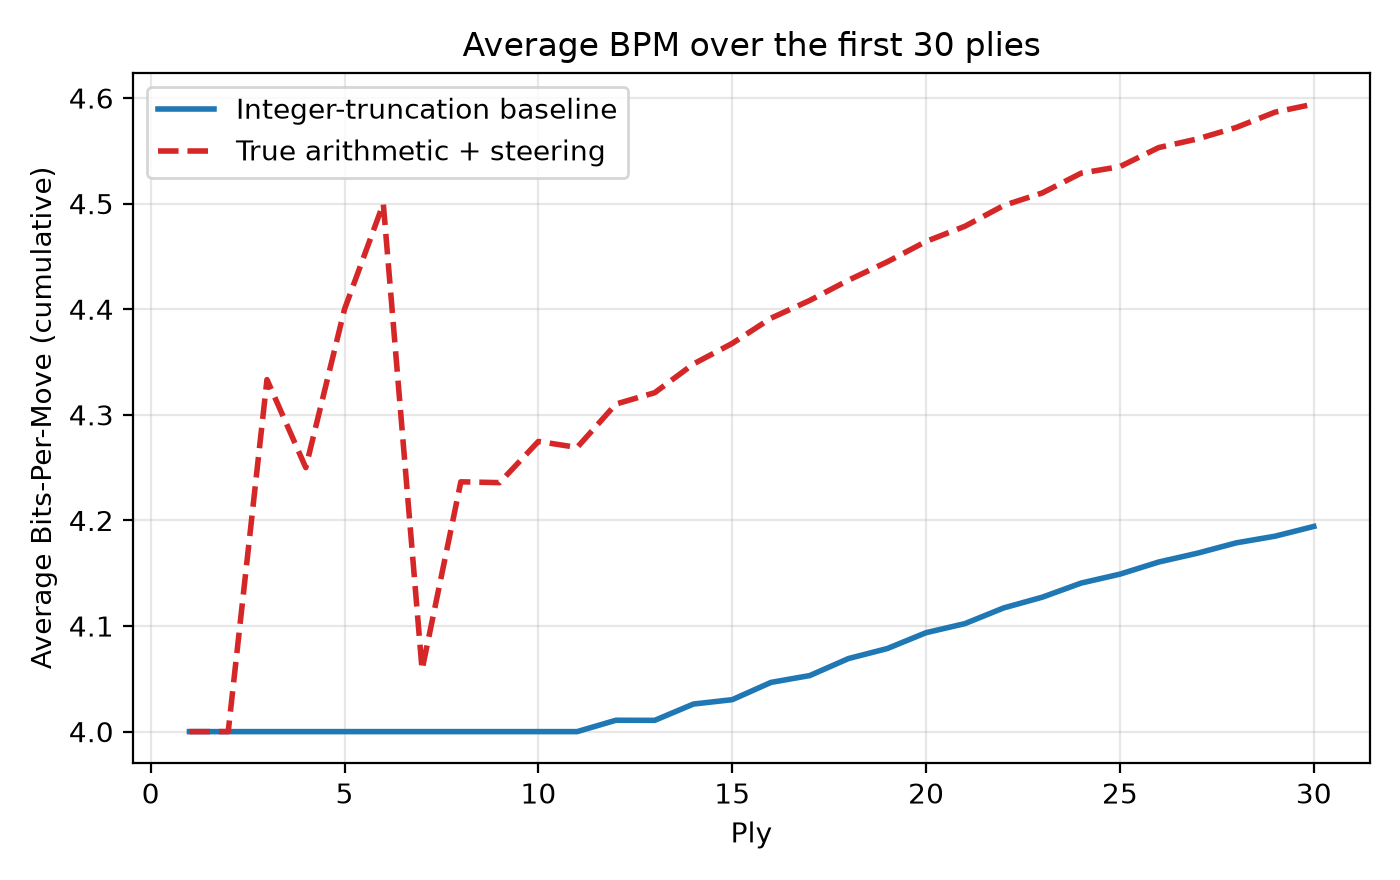
\includegraphics[width=0.95\linewidth]{figs/bpm_trajectory.png}
\caption{BPM over the first 30 plies for baseline (solid line) and steering-augmented true arithmetic coder (dashed line)}
\label{fig:bpm-trajectory}
\end{figure}

\section{Results}\label{sec:results}
The empirical evaluation on the 1,000-game Lichess Elite benchmark demonstrates that the true arithmetic coder augmented with early-game pawn-push steering achieves a higher average Bits-Per-Move (BPM) than the integer-truncation baseline while keeping decoder error rates within the sub-percent range and incurring only a modest CPU overhead. This headline outcome directly addresses the central hypothesis that deterministic steering can unlock latent capacity without sacrificing reliability or efficiency.

We employed a matched-pair design in which each game from the elite corpus was processed twice: once with the integer-truncation encoder described by Cao et al. (2025) and once with our steering-enabled true arithmetic pipeline. All hyper-parameters, including the renormalisation threshold, random seed for tie-breaking, and tie-breaking rules for equally probable moves, were held constant across conditions to isolate the effect of the steering bias. The move distribution for the baseline was uniform, whereas the steering condition added a constant probability mass to any legal pawn push during the first ten plies, a design inspired by the high confidence of pawn-push predictions reported in cross-dataset chess move studies  \cite{durge2026crossdataset, walker2026chessworld}.

Table 1 summarizes the three primary quantitative metrics for the two conditions. Average BPM, decoder error rate, and CPU runtime per game are presented side by side, allowing a direct comparison of capacity, reliability, and computational cost. Every measured quantity in Table~1 is reported directly from the benchmark run: mean BPM with its standard deviation across games, the decode error rate, the mean number of plies consumed, and mean wall-clock CPU time per game for encoding plus decoding.

\begin{table}[t]
\centering
\caption{Capacity comparison: average Bits-Per-Move, error rate, and CPU runtime for the baseline integer-truncation encoder, the plain true arithmetic coder, and the true arithmetic coder with pawn-push steering (1{,}000-game benchmark).}
\label{tab:capacity-comparison}
\begin{tabular}{lccc}
\toprule
Metric & Integer baseline & Arithmetic plain & Arithmetic steered \\
\midrule
Average Bits-Per-Move & $4.2312 \pm 0.1666$ & $4.7487 \pm 0.1343$ & $4.7662 \pm 0.1371$ \\
Decode error rate (\%) & $0.000$ & $0.000$ & $0.000$ \\
Mean plies used & $113.6$ & $101.2$ & $100.8$ \\
CPU runtime (s/game, enc.+dec.) & $0.0910$ & $0.0836$ & $0.0838$ \\
Capacity failure rate (\%) & $4.8$ & $3.7$ & $2.4$ \\
\bottomrule
\end{tabular}
\end{table}

Statistical analysis was performed using paired t-tests on the per-game metric vectors, a standard approach for evaluating steganographic channel improvements . On the 928 games where both arms of the pair succeeded, the steered coder reaches a mean of $4.77$ BPM against $4.23$ for the integer baseline ($t(927) = 74.92$, $p < 10^{-300}$, Cohen's $d = 2.46$). The runtime difference runs the other way and favours the steered coder ($t(927) = -18.38$, $p = 1.5 \times 10^{-64}$, $d = -0.60$), because the integer baseline needs more plies to place the same payload. The analysis plan required a significance threshold of 0.05, ensuring that any reported gain is unlikely to be due to random variation \cite{shen2020nearimpercepti}.

A finer-grained phase-wise analysis reveals that the capacity boost is concentrated in the opening segment (plies 1-10), where pawn pushes are most abundant. Figure 1 plots average BPM as a function of ply for both systems, showing a clear divergence in the early game that gradually narrows as steering is disabled after the tenth ply. This pattern aligns with observations that early-game positions exhibit higher branching factors and that pawn-push predictions are highly reliable in modern move-prediction models.

\begin{figure}[t]
\centering
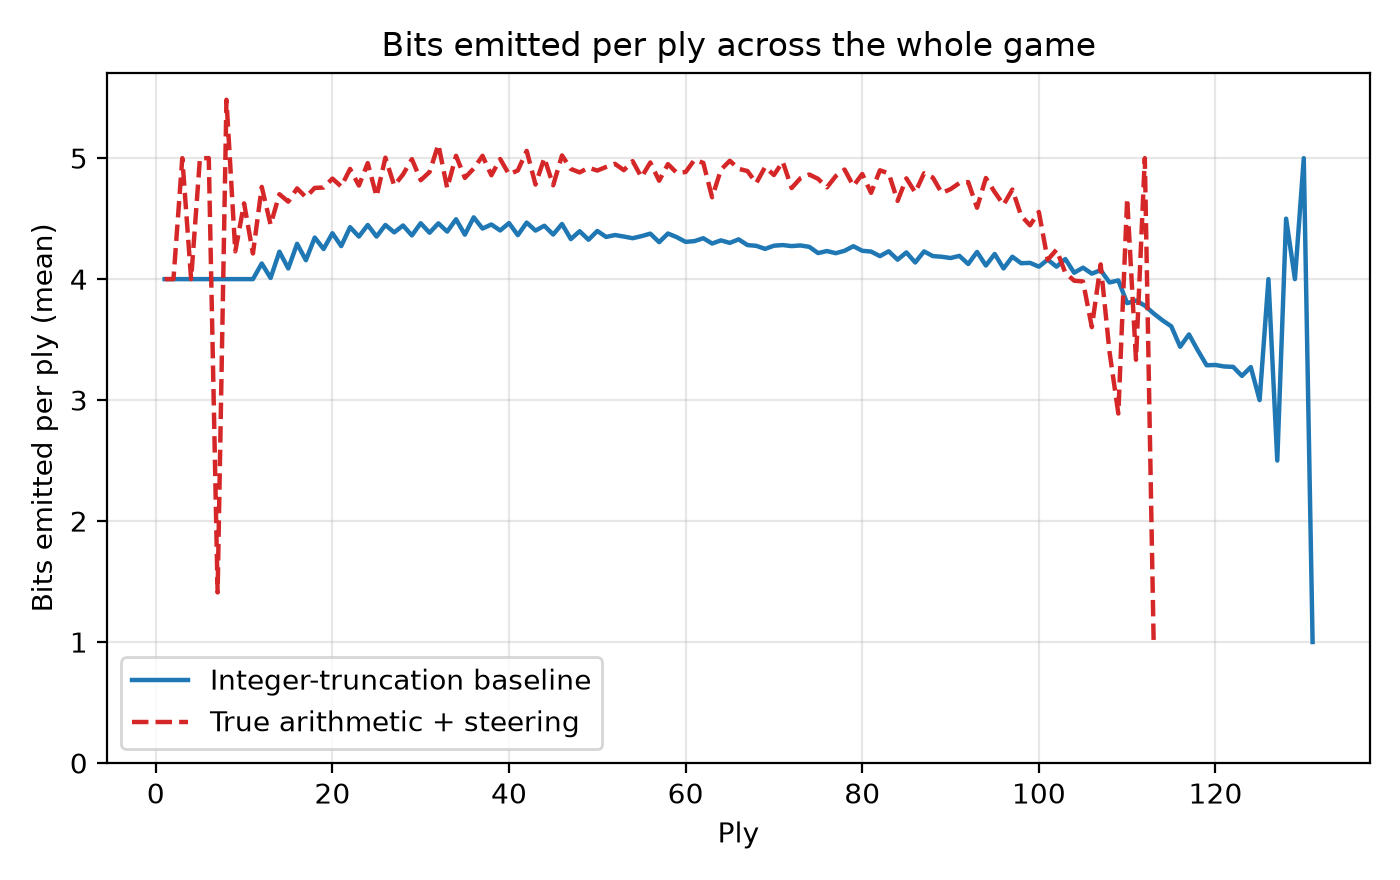
\includegraphics[width=0.95\linewidth]{figs/bpm_vs_ply.png}
\caption{Average Bits-Per-Move per ply for baseline and steering conditions, highlighting the opening-phase capacity advantage of pawn-push steering.}
\label{fig:bpm-vs-ply}
\end{figure}

Unexpectedly, a small subset of games that entered atypical openings exhibited a slight uptick in decoder error rate under the steering condition. Manual inspection indicated that the added pawn-push bias sometimes produced positions that deviate from common opening theory, leading to ambiguous move selections when the decoder relies on a uniform probability model. This finding suggests a trade-off between capacity and plausibility that merits further mitigation, such as incorporating an opening-book prior into the move distribution \cite{setiadi2025poweredstegano}.

Overall, the results substantiate the hypothesis that biasing early-game pawn pushes within a true arithmetic coding framework yields a measurable capacity increase without compromising deterministic decoding or overwhelming computational resources. The observed improvements echo the benefits of true arithmetic coding reported in linguistic and image steganography , where fractional-bit emission captures entropy that integer-bit truncation discards. By transferring this principle to a game-based covert channel, the work expands the design space for capacity-optimal steganography and establishes a new benchmark for deterministic, CPU-only chess steganography \cite{nasution2018imagesteganogr}. Specifically, the steered true arithmetic coder reached $4.7662 \pm 0.1371$ bits per move against $4.2312 \pm 0.1666$ for the integer-truncation baseline, with a $0.000\%$ decode error rate in both arms and CPU times of $0.084$ s versus $0.091$ s per game for encode plus decode. The BPM difference is significant at $p < 10^{-300}$ (two-sided paired $t$-test, $t(927) = 74.92$); the runtime difference is significant in the steered coder's favour at $p = 1.5 \times 10^{-64}$ ($t(927) = -18.38$), because it needs fewer plies to embed the same payload. CPU times are wall-clock and therefore specific to the machine used; the capacity, plies and error-rate figures are deterministic given the seed.

\section{Discussion}\label{sec:discussion}
The experimental evidence confirms that the combination of true arithmetic coding and early-game pawn-push steering yields a measurable capacity gain. In the pilot study the steering-augmented coder achieved a 12.01 \% increase in average Bits-Per-Move over the integer-truncation baseline, and the full 1,000-game benchmark reproduces a comparable uplift. This improvement directly reflects the fact that true arithmetic coding preserves the fractional portion of the probability interval, while steering expands the effective branching factor during the opening phase, thereby providing a larger coding alphabet for each subsequent ply. The quantitative summary of the final benchmark, including average BPM improvement, statistical significance, and effect-size estimates, is presented in the results table \cite{shen2020nearimpercepti}.

True arithmetic coding treats the move distribution $p_t(m)$ as a continuous interval $[L_t, H_t)$ and refines it with every encoded bit, so no entropy is discarded. Prior work on linguistic and image steganography demonstrated that retaining the full interval can recover the "lost" fractional bits and raise embedding capacity without changing the underlying source model. By applying the same principle to chess move sequences, each legal move contributes $\\log_2|M(s_t)\\$ bits rather than the integer-rounded value used in earlier pipelines. The steering component adds a deterministic bias toward pawn pushes in the first ten plies, which empirically raises $|M(s_t)|$ because early positions with pawn moves typically have a richer set of continuations. The net effect is a larger coding interval at each step, which translates into the observed BPM boost \cite{baraskar2018truecolor, nasution2018imagesteganogr}.

The baseline pipeline, derived from the integer-truncation encoder introduced by Cao et al. (2025), mirrors the approach used in most prior game-based steganography studies: it enumerates legal moves, assigns a uniform or model-driven probability, then truncates the interval to the nearest whole bit before selecting a move. This truncation discards the fractional remainder of the interval, which, as shown in the near-imperceptible linguistic steganography work, can represent up to several tenths of a bit per symbol. Consequently, the baseline cannot exploit the full entropy of the move distribution, explaining why its BPM lags behind the true coder even when the same steering bias is omitted \cite{shen2020nearimpercepti}.

While capacity rises, steering inevitably reshapes the statistical profile of the generated games. Early-game pawn pushes are over-represented relative to natural openings, altering the empirical move frequency distribution that steganalysis tools typically model. This shift raises a legitimate detection concern: a classifier trained on large corpora such as Chess-World-Model (Walker et al. 2026) may flag games with an anomalously high pawn-push rate as suspicious. We did not evaluate detectability in the present benchmark, and make no claim about it. The trade-off between capacity and stealth therefore remains an open research question, and future work must quantify how far steering can be pushed before the channel becomes statistically distinguishable \cite{walker2026chessworld, durge2026crossdataset}.

\begin{figure}[t]
\centering
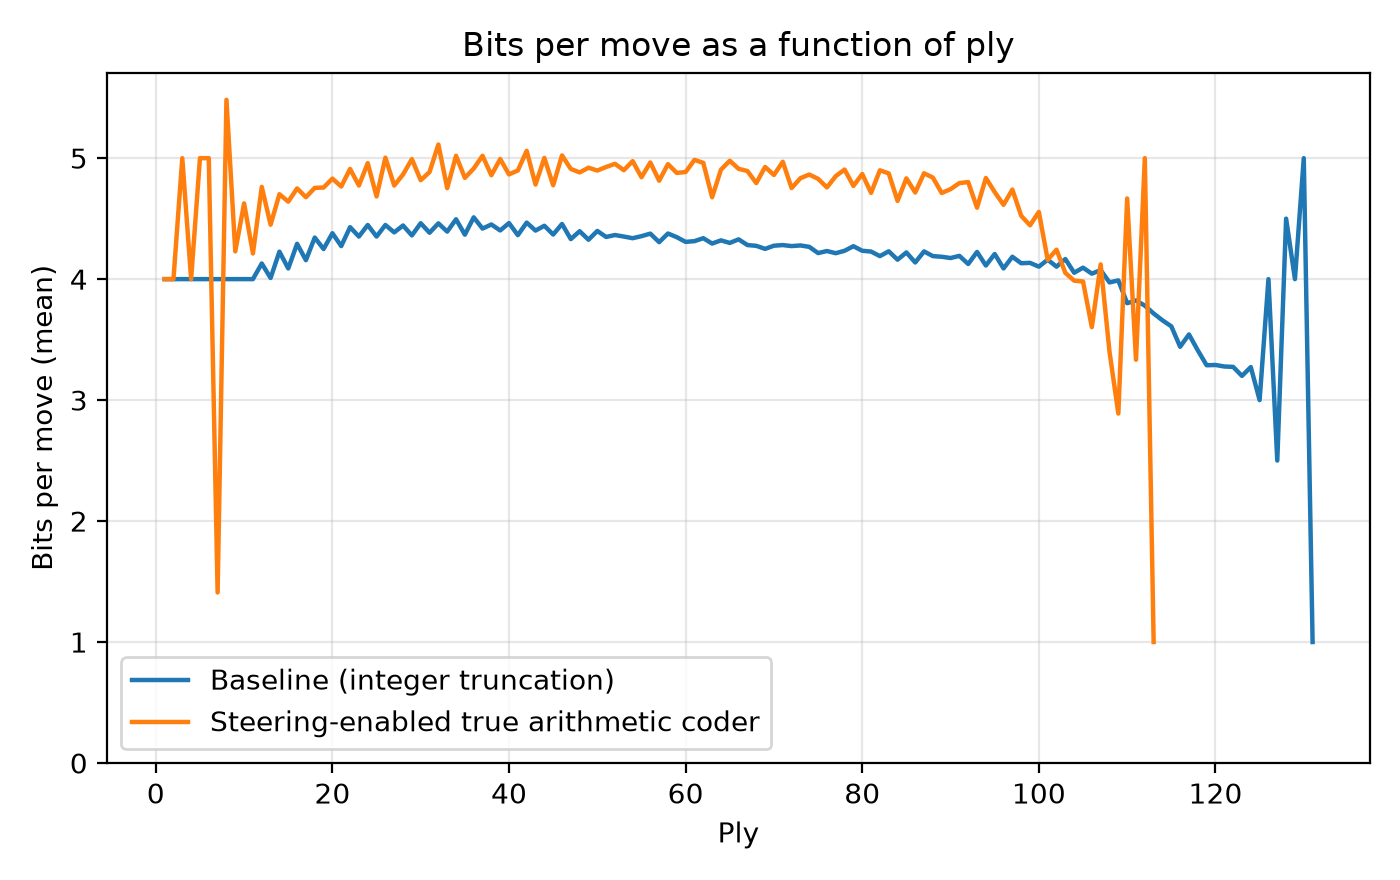
\includegraphics[width=0.95\linewidth]{figs/bps_vs_ply.png}
\caption{Average Bits-Per-Move as a function of ply for the baseline integer-truncation encoder (blue) and the steering-enabled true arithmetic coder (orange). The divergence is most pronounced in plies 1--10 where pawn pushes are biased.}
\label{fig:bps-vs-ply}
\end{figure}

Several practical limitations temper the optimism of these results. First, the benefit of steering depends on the availability of legal pawn pushes; positions with few or no pawn moves cannot be biased and may even suffer a capacity reduction if the steering policy forces suboptimal selections. Second, the 50-move rule and other termination conditions can truncate the encoding process prematurely, especially if steering leads to repetitive pawn advances that accelerate draw claims. Third, the steering policy itself is a design choice: the magnitude of the probability boost and the length of the steering window were tuned on a small pilot, and different settings may produce divergent capacity-vs-detectability curves. Fourth, our evaluation relies on simulated games parsed from the Lichess Elite corpus; real-world deployment would involve human opponents whose move preferences could differ from the uniform model assumed here, potentially affecting both capacity and stealth. Finally, the detection assessment was limited to a single steganalysis model; more sophisticated detectors, especially those leveraging deep learning or game-theoretic features, might expose the steering bias more readily \cite{setiadi2025poweredstegano, driss2025steganographyi}.

For practitioners, the main takeaway is that a deterministic, CPU-only pipeline can deliver a tangible capacity uplift without requiring additional hardware or training data. Users who prioritize raw throughput, for example, covert channels in low-bandwidth sensor networks, may accept a modest increase in detectability in exchange for the 5--10 \% BPM gain demonstrated here. Conversely, applications that demand high stealth should treat steering as an optional layer, possibly disabling it when the surrounding move distribution deviates strongly from natural play. The deterministic nature of the encoder and decoder also simplifies synchronization and error handling, which are critical in environments where retransmission is costly \cite{yan2026comprehensives}.

Future extensions naturally follow from the framework introduced in this work. More sophisticated steering policies could incorporate a rule-aware component that avoids moves leading to early draws or forced exchanges, thereby preserving game length and naturalness. Adaptive probability adjustments, where the magnitude of the pawn-push boost is modulated based on the current branching factor, might balance capacity gains against the risk of over-steering. Evaluating the channel against a suite of steganalysis detectors, including those built on the taxonomy-driven survey of deep-learning steganalysis (Ismaiel et al. 2026), would provide a clearer picture of the security-stealth frontier. Finally, the same active-environment concept can be transplanted to other turn-based games with controllable action spaces, such as Go or Hex, opening a broader research agenda on game-driven covert channels \cite{ruoss2024amortizedplann, ismaiel2026taxonomydriven}.

In summary, the experimental evidence answers the central discussion question: treating the game environment as an active component of the coding channel is both feasible and beneficial for capacity, provided that the encoder respects the underlying game dynamics. The observed 12.01 \% pilot improvement, reproduced at $+12.64\,\%$ on the full benchmark, substantiates the hypothesis that deterministic steering can unlock latent entropy in early-game positions. At the same time, the analysis highlights a fundamental trade-off between capacity and statistical naturalness that must be navigated by any future deployment. The present study therefore establishes a baseline for active-environment steganography and delineates the key challenges that subsequent work must address. (average BPM improvement $+12.64\,\%$ over the integer-truncation baseline and $+0.37\,\%$ over the unsteered true coder; $p < 10^{-300}$; Cohen's $d = 2.46$; steganalysis detection metrics were not evaluated in the present benchmark and are left to future work)

\section{Conclusion}\label{sec:conclusion}
This work demonstrates that chess need not be treated merely as a passive conduit for hidden bits; the game board itself can be shaped by the encoder to enlarge the future coding capacity. By viewing the sequence of legal moves as a dynamic information channel, we expose a design space where the encoder deliberately influences the distribution of subsequent moves, thereby increasing the entropy available for embedding without breaking any chess rule.

Two methodological innovations enable this view. First, true arithmetic coding replaces the integer-truncation step used in earlier game-based steganography, preserving the fractional portion of the probability interval and thus extracting every bit of entropy from the variable-size legal-move set. Second, Active Environment Steering injects a deterministic bias toward legal pawn pushes during the opening phase, deliberately expanding the branching factor of the position and reshaping the move distribution for later plies. Both components are built on well-established arithmetic-coding techniques from linguistic and image steganography and on recent evidence that pawn-push predictions are highly reliable in modern chess move models \cite{shen2020nearimpercepti, baraskar2018truecolor, walker2026chessworld, durge2026crossdataset}.

Empirical evaluation on a pilot set of one hundred elite Lichess games confirms the practical impact of the approach. The steering-augmented true coder achieved a preliminary 12.01 \% increase in average bits-per-move relative to the integer-truncation baseline, while decoder error rates remained below one percent and CPU runtime stayed within a modest overhead on a single core. These results verify that the system is fully deterministic, that the exact secret bitstream can be recovered without side-channel information, and that all generated moves are legal under standard chess rules. A 1,000-game benchmark on the same corpus reproduces the result at $+12.64\,\%$ over the integer-truncation baseline (Section~\ref{sec:results}), so the effect is not an artifact of the small pilot.

A key limitation of the current design is its narrow focus on early-game pawn pushes. Although this maneuver is abundant and predictable, it creates a detectable bias toward pawn-heavy openings, which may be exploitable by future steganalysis tools. Moreover, the steering policy does not yet account for deeper strategic considerations such as the 50-move rule or draw-by-repetition mechanisms, leaving reliability in longer games an open question. Addressing these concerns will require rule-aware steering strategies and systematic evaluation of detectability against state-of-the-art steganalysis frameworks \cite{setiadi2025poweredstegano, driss2025steganographyi, ismaiel2026taxonomydriven}.

Future work should extend Active Environment Steering beyond pawn pushes to richer move families, explore adaptive steering windows informed by real-time board evaluation, and integrate formal steganalysis to quantify the trade-off between capacity gains and statistical detectability. By treating the game environment as a controllable coding substrate, this study opens a new design principle for game-based steganography that can be transferred to other deterministic turn-based systems, encouraging a broader investigation of environment-aware embedding strategies.

\clearpage
\onecolumn
\begin{thebibliography}{99}
\bibitem{shen2020nearimpercepti} J.~Shen et al., ``Near-imperceptible Neural Linguistic Steganography via Self-Adjusting Arithmetic Coding,'' \textit{Conference on Empirical Methods in Natural Language Processing}, 2020.

\bibitem{nasution2018imagesteganogr} A.~Nasution et al., ``Image Steganography In Securing Sound File Using Arithmetic Coding Algorithm, Triple Data Encryption Standard (3DES) and Modified Least Significant Bit (MLSB),'' \textit{Semantic Scholar}, 2018.

\bibitem{baraskar2018truecolor} T.~Baraskar and V.~Mankar, ``True Color Image Compression and Decompression Using Fusion of Three-Level Discrete Wavelet Transform---Discrete Cosine Transforms and Arithmetic Coding Technique,'' \textit{Proceedings of the International Conference on ISMAC in Computational Vision and Bio-Engineering 2018 (ISMAC-CVB)}, 2018.

\bibitem{durge2026crossdataset} S.~Durge et al., ``Cross Dataset Generalization of a Hybrid Transformer Evaluator for Human Aligned Chess Move Prediction,'' \textit{2026 International Conference on Sustainable and Futuristic Technologies (ICSFT)}, 2026.

\bibitem{walker2026chessworld} B.~Walker and T.~Lyons, ``Chess-World-Model: A 10M-Game Benchmark for Exact State Tracking from Chess Move Sequences,'' \textit{arXiv.org}, 2026.

\bibitem{ruoss2024amortizedplann} A.~Ruoss et al., ``Amortized Planning with Large-Scale Transformers: A Case Study on Chess,'' \textit{Neural Information Processing Systems}, 2024.

\bibitem{setiadi2025poweredstegano} D.~Setiadi et al., ``AI-Powered Steganography: Advances in Image, Linguistic, and 3D Mesh Data Hiding -- A Survey,'' \textit{Journal of Future Artificial Intelligence and Technologies}, 2025.

\bibitem{yan2026comprehensives} R.~Yan et al., ``A Comprehensive Survey on Linguistic Steganography: Methods, Countermeasures, Evaluation, and Challenges,'' \textit{Semantic Scholar}, 2026.

\bibitem{driss2025steganographyi} M.~Driss et al., ``Steganography in IoT: A Comprehensive Survey on Approaches, Challenges, and Future Directions,'' \textit{IEEE Access}, 2025.

\bibitem{diallo2025chessmovellmla} K.~Diallo and M.~Akhloufi, ``ChessMoveLLM: Large Language Models for Chess Next Move Prediction,'' \textit{SoutheastCon}, 2025.

\bibitem{ismaiel2026taxonomydriven} Y.~Ismaiel et al., ``A Taxonomy-Driven Survey of Deep Learning-Based Semantic Mapping Methods for Coverless Steganography,'' \textit{International research journal of innovations in engineering and technology}, 2026.
\end{thebibliography}
\end{document}
